69. \begin{figure}[ht!]
\center{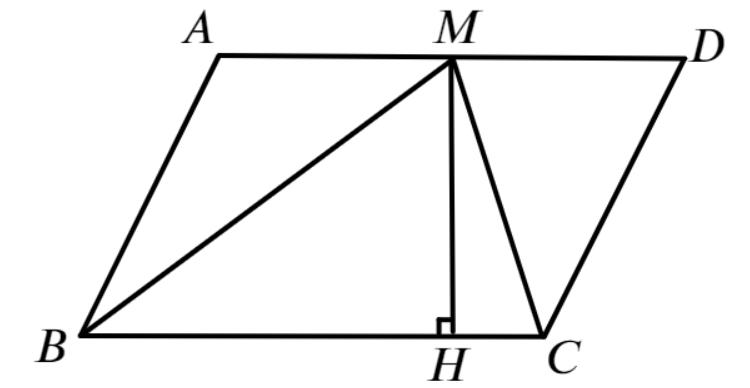
\includegraphics[scale=0.35]{g8-69.png}}
\end{figure}\\
Проведём перпендикуляр $MH,$ он является высотой треугольника и равен высоте параллелограмма. Так как $S_{\Delta MCB}=\cfrac{1}{2}MH\cdot CB,$ а $S_{ABCD}=MH\cdot CB,$ площадь параллелограмма в 2 раза больше и равна $2\cdot42=84\text{ см}^2.$\\
